\begin{theorem}{(60, 61)} Process life cycles (Figure \ref{img:process_lifecycles}): \begin{itemize}
        \item State:\begin{itemize}
            \item New (Created):Process is created and PCB is allocated in kernel, but memory space is NOT allocated.
            \item Ready:Process is allocated memory space.
        \end{itemize}
        \item Zombie state:Process is finished, but the parent process have NOT collected results of the children processes, or parent process have NOT executed \code{wait()} system call. Resources are released, but PCB have NOT been deleted, until parent process collects the results, then kernel delete PCB.
    \end{itemize}
\end{theorem}

\begin{figure}[H]
    \centering
    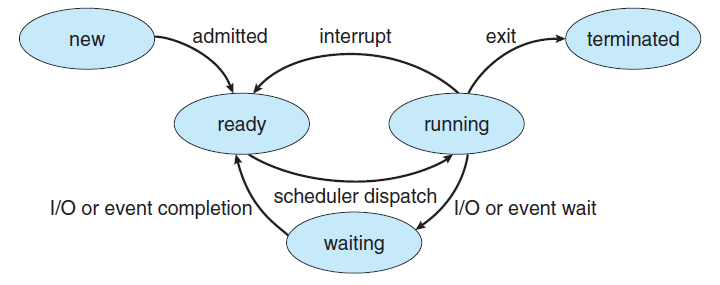
\includegraphics[scale=0.8]{img/process_lifecycles.png}
    \caption{Process life cycles.}
    \label{img:process_lifecycles}
\end{figure}

\begin{theorem}{(67)} Scheduler:\begin{itemize}
        \item Long-term (Job) scheduler:通常僅\textbf{batch system採用},從job queue中選jobs載入memory。執行頻率最低,可以調控multiprogramming degree與CPU-bound與I/O-bound jobs的比例。
        \item Short-term (CPU, process) scheduler:從ready queue選擇一個process分派給CPU執行。\textbf{所有系統都需要},執行頻率最高,\textbf{無法}調控multiprogramming degree與CPU-bound與I/O-bound jobs的比例。
        \item Medium-term scheduler:Memory space不足且有其他processes需要更多memory時執行,選擇Blocked或lower priority process swap out to disk。僅\textbf{Time-sharing system採用},batch和real-time systems不採用,可以調控multiprogramming degree與CPU-bound與I/O-bound jobs的比例。
    \end{itemize}
\end{theorem}

\begin{theorem}{(70)} Dispatcher: \begin{itemize}
        \item 將CPU真正分配給CPU scheduler選擇的process。
        \item Context switch.
        \item Switch mode to user mode.
        \item Jump to execution entry of process.
    \end{itemize}
\end{theorem}

\begin{theorem}{(63)} \code{execlp(dir, filename, args)}:載入特定工作執行,memory content不再是parent process的複製,沒有參數填\code{NULL},
    e.g. \code{execlp("/bin/ls", "ls", NULL)}。
\end{theorem}

\begin{theorem}{(71, 72, 75, 76, 77, 78)} Scheduling algorithms: \begin{itemize}
        \item FCFS (First-come-first-serve):可能遭遇\textbf{Convoy effect},即許多processes都在等待一個需要很長CPU time的process完成工作。
        \item SJF (Shortest-Job-First):\begin{itemize}
            \item Preemptive SJF又稱SRTF (Shortest-Remaining Time First)。
            \item 效益最佳(包含SRTF),即平均等待時間最短。
        \end{itemize}
        \item Round-Robin (RR) scheduling:平均turnaround time\textbf{未必}會隨著quantum time增加而下降。
        \item Multi-level queue (MQ):易starvation,且無法通過類似Aging改善。
        \item Multi-level feedback queue (MFQ):可以採用類似Aging防止starvation。
        \item Priority scheduling:\begin{equation}
            \begin{aligned}
                \text{FCFS}, \text{SJF}, \text{SRTF} & \subset \text{Priority} \\
                \text{FCFS} & \subset \text{RR} \\
                \text{FCFS}, \text{SJF}, \text{SRTF}, \text{Priority}, \text{RR}, \text{MQ} & \subset \text{MFQ}
            \end{aligned}
        \end{equation}
        \begin{table}[H]
            \centering
            \begin{tabular}{|c|c|c|c|c|}
                \hline
                Scheduling & 公平 & Preemptive & Non-preemptive & Starvation \\
                \Xhline{2\arrayrulewidth}
                FCFS & $\surd$ & & $\surd$ & \\
                \hline
                SJF & & & $\surd$ & $\surd$ \\
                \hline
                SRTF & & $\surd$ & & $\surd$ \\
                \hline
                Priority & & $\surd$ & $\surd$ & $\surd$\\
                \hline
                RR & $\surd$ & $\surd$ & & \\
                \hline
                MQ & & $\surd$ & & $\surd$ \\
                \hline
                MFQ & & $\surd$ & & \\
                \hline
            \end{tabular}
        \end{table}
    \end{itemize}
\end{theorem}

\begin{theorem}{(80)} Prioity inversion:Higher priority process waits for lower priority process to release resources. 通過Priority inheritance解決:讓lower priority process暫時繼承higher priority,以便盡快取得CPU執行,完成後再恢復lower priority。
\end{theorem}

\begin{theorem}{(80)} Hard real-time system:\begin{itemize}
        \item Schedulable判斷:\begin{equation}
            \sum_{i = 1}^{n} \frac{c_i}{p_i} \le 1
        \end{equation} 若符合則schedulable。其中,$n$為事件數目,$c_i$為CPU burst time,$p_i$為period time。
        \item Process meets deadline scheduling algorithms:\begin{itemize}
            \item Rate-Monotonic:\begin{itemize}
                \item Static priority且preemptive。
                \item Period time越小,則priority越高。
                \item Under schedulable,也\textbf{不能}保證所有event皆滿足deadline。
                \item 若其無法滿足deadline,其他static priority scheduling也無法。
            \end{itemize}
            \item EDF (Earliest Deadline First):\begin{itemize}
                \item Dynamic priority且preemptive。
                \item Deadline越小,則priority越高。
                \item Under schedulable,保證所有event皆滿足deadline。
                \item CPU utilization不可能達到$100\%$。
            \end{itemize}
        \end{itemize}
    \end{itemize}
\end{theorem}

\begin{theorem}{(86)} Thread:\begin{itemize}
        \item process是OS分配\textbf{resources}的基本單位,而thread是OS分配\textbf{CPU time}的基本單位。
        \item 同一process之threads共享process的data section (static local and global variables)、heap和code section等,在同一個address可以有多個threads同時執行。
        \item 同一process的不同threads可以平行在不同CPUs上執行。
        \item 種類:\begin{itemize}
            \item User-level thread:\begin{itemize}
                \item 由在user site的thread library管理,不需要kernel管理,e.g. POSIX的pthread library,但只是提供規格並沒有實現。
                \item Kernel不知道其存在,因此kernel不干預,導致不同threads\textbf{無法}平行在不同CPUs上執行。
                \item 若user thread發出blocking system call時,則該process也會被blocked,即時該process還有其他available threads。
            \end{itemize}
            \item Kernel-level thread:現行OS皆支持,e.g. Windows Thread library and Java Thread library。
        \end{itemize}
    \end{itemize}
\end{theorem}

\begin{theorem}{(88)} Thread model (user thread-to-kernel thread):\begin{itemize}
        \item Many-to-One model:即user-level thread。
        \item One-to-One model:\begin{itemize}
            \item Not efficient than Many-to-One model.
            \item e.g. Linux, family of Windows OS, OSX.
        \end{itemize}
        \item Many-to-Many model:\begin{itemize}
            \item Overhead較One-to-One小,但製作較複雜。
            \item NOT efficient than Many-to-One model.
            \item e.g. Solaris 2,但它是用two-level mapping model製作,同時也允許One-to-One。
        \end{itemize}
    \end{itemize}
\end{theorem}
